\section{Future Direction and Limitations}
\label{sec:future}
The most obvious take away from the results displayed above is the
weakness of Flood in singleplayer and in low-energy environments.
This is mainly because of Flood's orientation: Flood was designed as
an aggressive, field-capturing organism and optimised for multi-player
fields with moderate to high resource levels.

Strategies to adjust Flood to each of these scenarios are described in
the following sections.
\subsection{Single-Player}
As a highly-aggressive quick-board-covering strategy is necessary for
multi-player scenarios, this would need to be Flood's default
behavior. After several rounds, it could identify whether or not the
board truly is multi-player and adjust the strategy accordingly.

One way to do this would be to use the state to keep track of the
number of turns passed and the whether or not enemies had been
detected:
\begin{verbatim}
	//if state = 0, enemy has been detected
	for (i=0 to 4) {
		if (neighbors(i) != -1 || neighbors(i) = 0) state = 0;
	} if (state != 0) state++;
\end{verbatim}

Using this algorithm, any organism that encounters either an enemy or
a friendly organism that has encountered an enemy has a record of that
interaction.

One method to adopt the PatternMaker strategy would be to allow a
random genetic mutation if enough turns have passed and no enemy is
encountered; that is, if state reaches a given threshold.  At this
point, a genetic mutation could be ��allowed��, in that it affects a
very small, random sample of organisms, causing them to adopt
PatternMaker behavior.  Should any non-PatternMaker organisms
encounter a Patternmaker, they should avoid the PatternMaker organism
and pursue self-destructive behavior (ie, avoid food and move often)
to try to clear the board for the PatternMaker��s entrance.

\begin{figure}[t]
\centering
  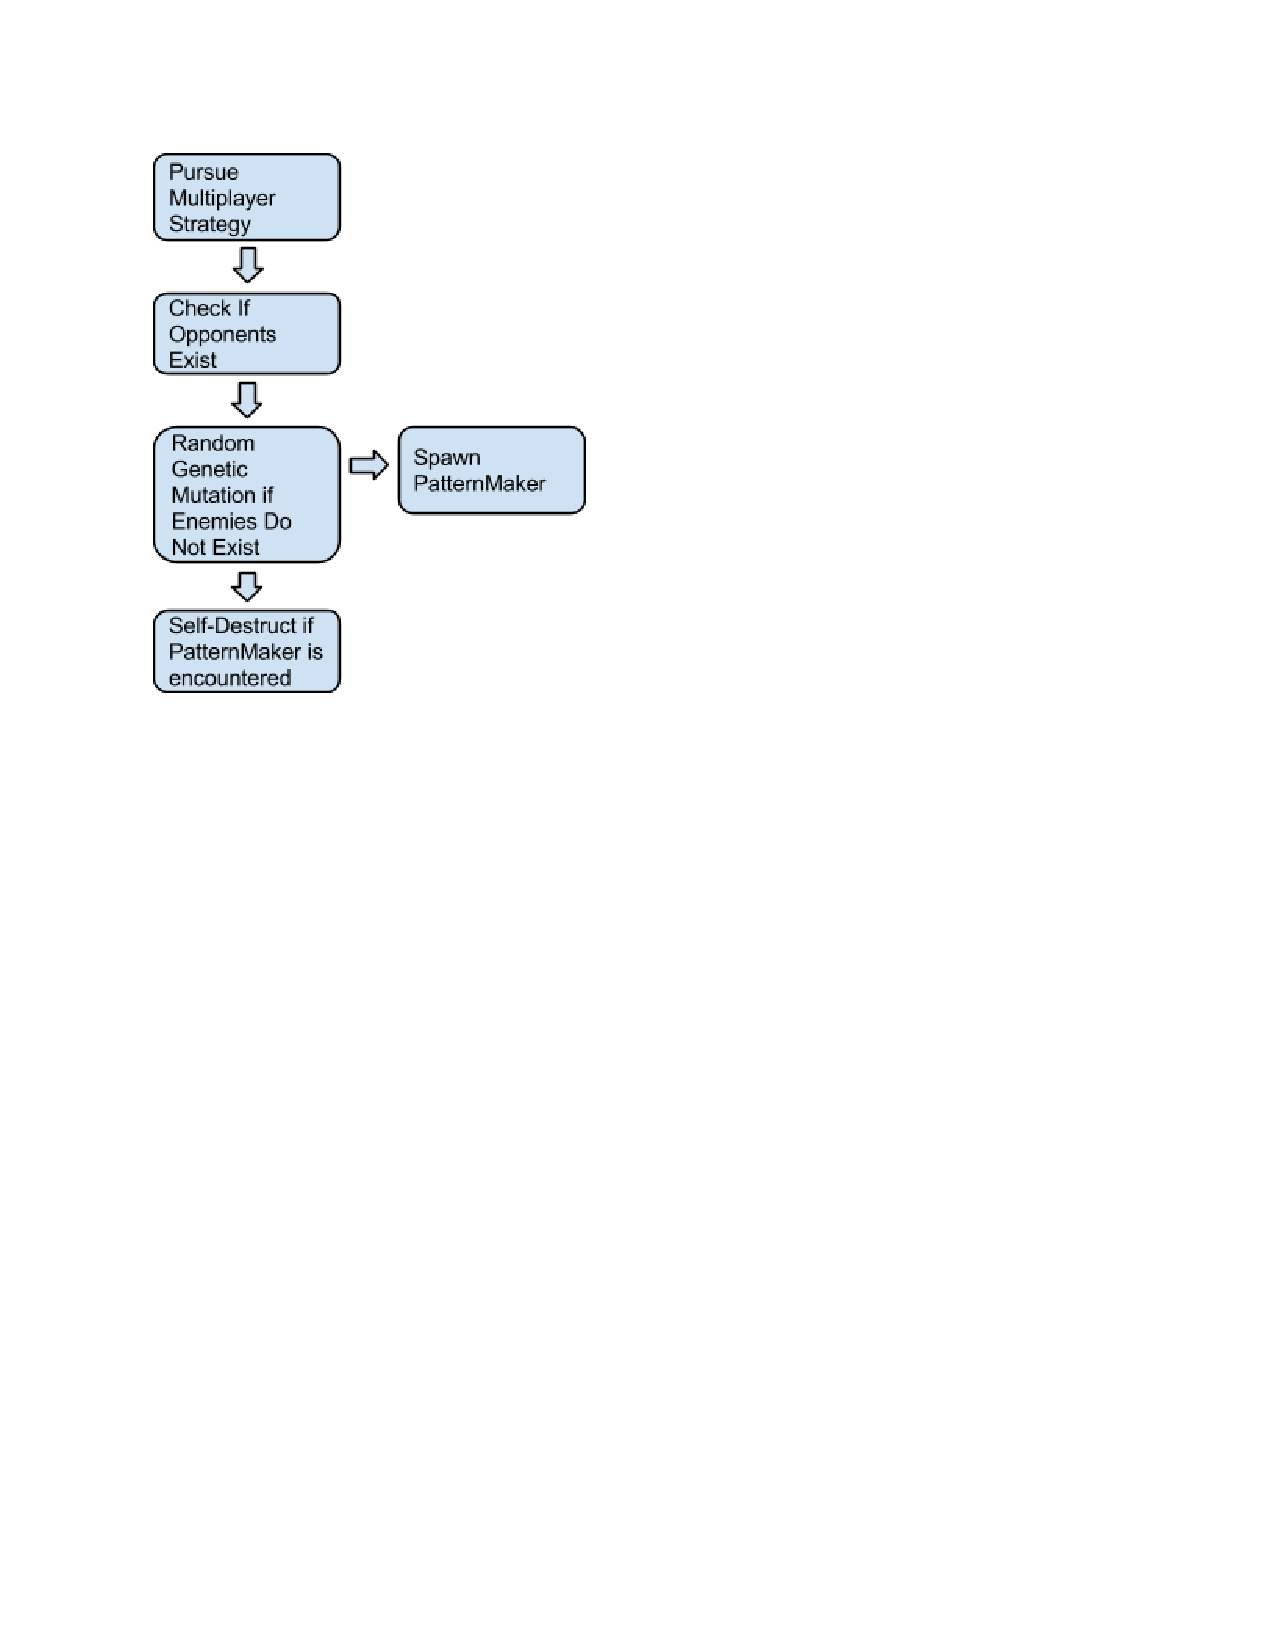
\includegraphics[trim=10mm 160mm 96mm 30mm]{figs/future-flowchart.pdf}\\
  \caption{Flowchart of potential future design}\label{fig:future-flowchart}
\end{figure}

Of course, this strategy does rely on a random element, but given a
sufficiently long game, it should serve as an effective transition to
a single-player strategy.

\subsection{Low Resources}
As Flood is a highly aggressive organism, it moves far and often,
especially early in the game.  In low-energy situations, this is very
undesirable and leads to extinction.

While prefixing Flood with Talker-type scouts would identify
low-energy conditions, this would also adversely affect Flood's
multi-player performance, as early board domination is a key part of
its strategy.

One way to handle low resources could be an envolution of PatternMaker
which give it the ability to make different patterns based on the
environmental conditions. Since we have the surviving mode completely
isolated from the energy maximization algorithm, the future work only
need to focus on establishing a better pattern for achieving a high
sustainable total energy.
